\section*{Log ud}
Log ud inddeles i en grænseflade og en dertilhørende controller, som det fremgår af \autoref{fig:MVCLogUd}. 

\begin{figure} [H]
\centering
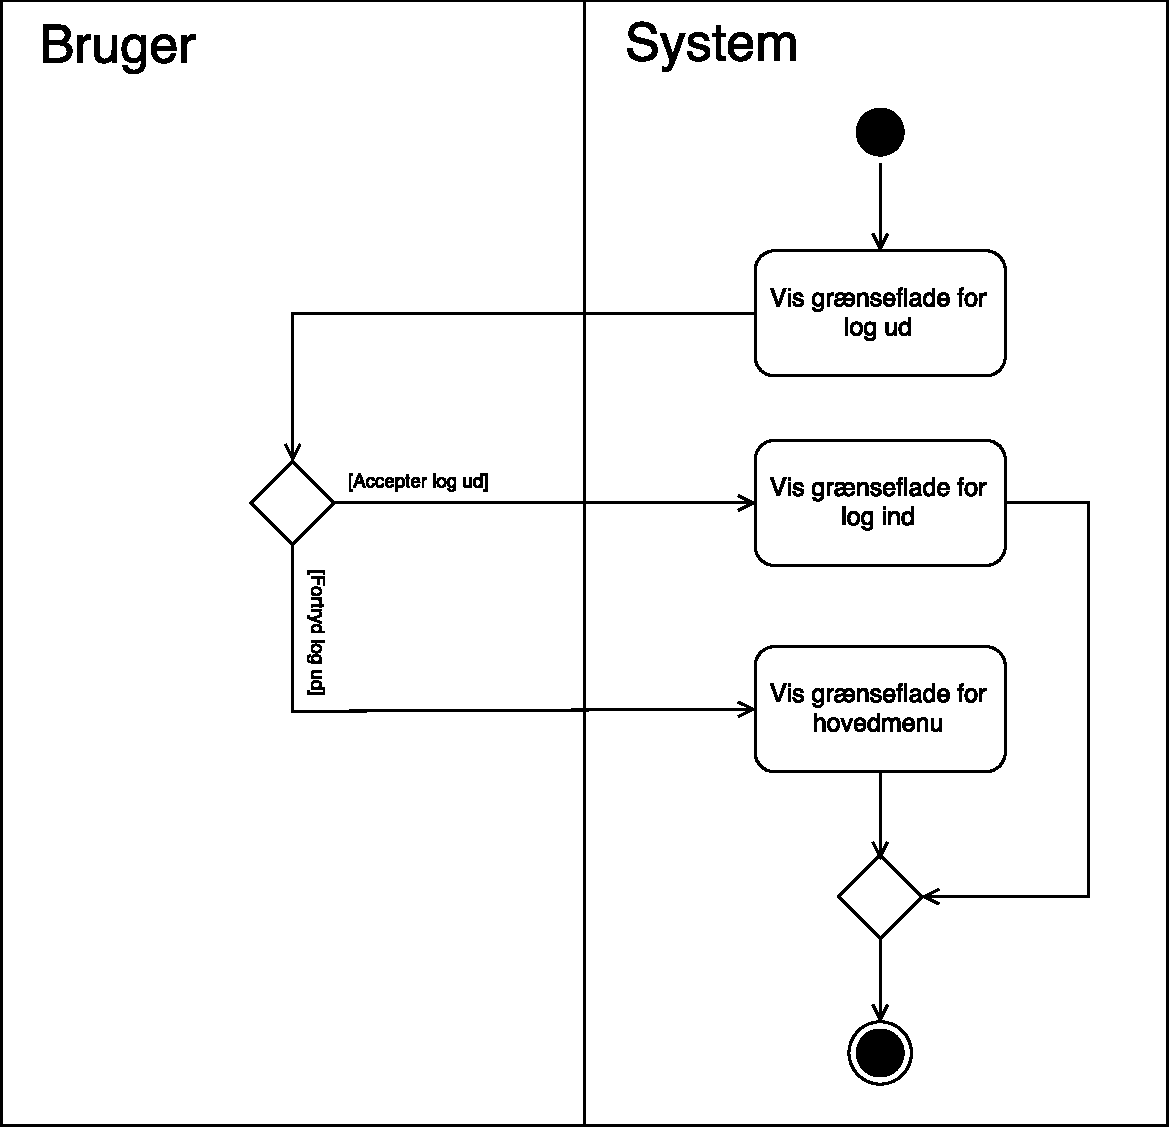
\includegraphics[width=0.6\textwidth]{figures/MVC/Logud}
\caption{Designklasser for log ud.}
\label{fig:MVCLogUd}
\end{figure}

\noindent
Der opstilles i \textit{LogudGrænseflade} et tekstfelt for log ud. Dertil opstilles en OK eller tilbage knap af typen button. 

Der er til \textit{LogudGrænseflade} opstillet en \textit{LogudController}, der har til formål at lytte til OK eller tilbage knap. Hvis brugeren trykker på OK knappen afsluttet forbindelse til databasen og skærmen for log ind vises. Hvis brugeren trykker på tilbage knappen vises hovedmenuen. Glemmer brugeren at logge ud startes en timer derved inaktivitet i længere tid logger brugeren ud. 